\documentclass{beamer}

\let\val\undefined
\usepackage{amsmath}
\usepackage{amsthm}
\usepackage{amsfonts}
\usepackage{grffile}
\usepackage{graphicx}
\usepackage{bm}

\usetheme[progressbar=frametitle]{metropolis}
%\usepackage{libertine}

% *** Styles ***
%\setbeamertemplate{navigation symbols}{}
%\usecolortheme{dolphin}
%\usecolortheme{rose}
%\setbeamercovered{transparent}
%\usefonttheme{professionalfonts}
%\usefonttheme[onlymath]{serif}

% *** Colors ***
\newcommand{\tc}[2]{\textcolor{#1}{#2}}
\newcommand{\tcb}[1]{\tc{blue}{#1}}
\newcommand{\tcr}[1]{\tc{red}{#1}}
\newcommand{\tcg}[1]{\tc{green}{#1}}

\def\checkmark{\tikz\fill[scale=0.4](0,.35) -- (.25,0) -- (1,.7) -- (.25,.15) -- cycle;}

\newcommand{\Ex}{\mathbb{E}}
\newcommand{\E}[1]{\mathbb{E}\left[#1\right]}
\newcommand{\Real}{\mathbb{R}}
\newcommand{\V}[1]{\mathbb{V}\left[#1\right]}
\newcommand{\I}{\mathbb{I}}
\newcommand{\sd}[1]{\operatorname{sd}\left[#1\right]}
\newcommand{\cov}[1]{\operatorname{Cov}\left[#1\right]}
\newcommand{\corr}[1]{\operatorname{corr}\left[#1\right]}
\renewcommand{\P}[1]{\mathbb{P}\left[#1\right]}


\title{Statistics and Normal Distribution}
\subtitle{MML 6.4-5}
\author{Marek Petrik}
\date{9/05/2023}

\begin{document}
\begin{frame}
\maketitle
{\tiny Some figures courtesy of the textbooks: ISLR and MML}
\end{frame}


\begin{frame} \frametitle{Important Properties}
  Marginalization
  \[
   \P{X = x}\;=\; \sum_{y\in \mathcal{T}} \P{X = x, Y = y} 
 \]
 Conditional probability
  \[
    \P{ X = x \mid Y = y } \; =\;  \frac{\P{ X = x, Y = y }}{\P{ Y = y }}
  \] 
  Product rule
  \[
     \P{ X = x, Y = y } \; =\;  \P{ X = x \mid Y = y } \cdot \P{ Y = y }
  \] 
  Independent random variables
  \[
    \P{ X = x,Y = y } = \P{ X = x } \cdot  \P{ Y = y }
  \]
  Bayes Theorem
  \[
   \P{ X = x \mid Y = y } =
    \frac{\P{ Y = y \mid X = x } \cdot \P{ X = x }}{\P{ Y = y }}
  \]
\end{frame}

\begin{frame} \frametitle{Conditional Independence}
Random variables $X,Y \colon \Omega \to \Real$ are \textbf{independent conditionally} on a random variable $Z$ if for all $x,y,z \in \Real$:
\[\P{ X = x,Y = y \mid Z = z} = \P{ X = x \mid Z = z} \cdot  \P{ Y = y \mid Z = z} \]
Examples?\\
\vspace{4cm}
\end{frame}

\begin{frame}\frametitle{Continuous Probability Distributions} 
    \begin{itemize}
    \item \textbf{Normal}: common because of central limit theorem
    \item \textbf{Laplace}: Extreme weather events
    \item \textbf{Multivariate normal}: Height and weight
    \end{itemize}
  {\small See Wikipedia for their properties}
\end{frame}

\begin{frame} \frametitle{Cumulative Distribution Function}
  \[
    F_X(x) \; =\;  \P{X \le x} = 
    P \left( \left\{ \omega \in  \Omega \mid X(\omega) \le x \right\} \right)
  \]
  Example: Uniform random variable on $[0,1]$
  \vspace{5cm}
\end{frame}

\begin{frame} \frametitle{Probability Density Function}
  Function $f_X\colon \Real \to \Real$ is a pdf of $X$ if $\forall x$
  \[
   F_X(x)  = \int_{-\infty}^x f_X(t) dt 
 \]
 \vspace{4cm}
\end{frame}

\begin{frame} \frametitle{Conditional Probability Density Function}
  For random variables $X, Y$ with a joint density $f_{X,Y}\colon \Real^2 \to \Real$, the conditional density is (when $f_X(x) > 0$):
  \[
   f_{Y \mid X}(y \mid  x) = \frac{f_{X,Y}(x,y)}{f_X(x)}
 \]
 \vspace{4cm}
\end{frame}

\begin{frame} \frametitle{Today}
  \begin{enumerate}
  \item Expected value
  \item Variance, covariance, and correlation
  \item Normal distribution
  \end{enumerate}
\end{frame}


\begin{frame} \frametitle{Expected Value (Mean)}
  Random variable $X$ (discrete and continuous, see Lebesgue integrals)
  \[
   \E{X} = \sum_{x\in \mathcal{X}} x \cdot \P{X = x},  \qquad  \E{X} = \int_{\Omega } X dP 
  \]
  \vspace{5cm}
\end{frame}

\begin{frame} \frametitle{Expected Value of Function}
  Random variable $X$ (discrete and continuous) and a function $g$
  \[
    \E{g(X)} = \sum_{g\in \mathcal{G}} g \cdot \P{g(X) = g},  \qquad
    \E{X} = \int_{\Omega } g(X) dP 
 \]
 \textbf{ Law of the Unconscious Statistician} proves that:
  \vspace{5cm}
\end{frame}

\begin{frame} \frametitle{Expected Value: Properties}
  Assume real-valued random variables $X$ and $Y$
  \[ \E{ c\cdot X } = c \cdot  \E{ X } \]
  \vfill
  \[ \E{ X + Y  } = \E{ X } + \E{ Y } \]
  \vfill
  When $X$ and $Y$ are \textbf{independent}:
  \[ \E{ X \cdot Y  } = \E{ X } \cdot \E{ Y } \]
\end{frame}

\begin{frame} \frametitle{Conditional Expectation}
  {\small \url{https://en.wikipedia.org/wiki/Conditional_expectation}}
  Conditioning on an event $A \in \mathcal{F}$ (discrete r.v.)
  \[
  \E{X \mid  A} \quad =\quad  \sum_{x\in \mathcal{X}} x \cdot \P{X=x \mid A} 
  \]
  \vfill
  Conditioning on a random variable $Y$:
  \[
   \E{X \mid Y} \colon \Omega \to \Real 
 \]
 defined as (discrete)
 \[
  \E{X \mid Y}(\omega) \quad =\quad  \sum_{x\in \mathcal{X}} x \cdot \P{X=x \mid Y = Y(\omega)} 
 \]
\end{frame}

\begin{frame} \frametitle{Expected Utility Theory}
  Two possible investments with profits $X_1$ and $X_2$ \\
  \vfill
  Choose investment one if
  \[ \E{ X_1 } \ge \E{ X_2 } \]
\end{frame}

\begin{frame} \frametitle{Monty Hall Problem}
  {\small \url{https://en.wikipedia.org/wiki/Monty_Hall_problem}}
\vfill 
  \begin{center}
    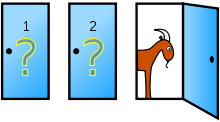
\includegraphics[width=0.7\linewidth]{../figs/prob/monty_hall.png}
  \end{center}
  \vfill 
\end{frame}

\begin{frame} \frametitle{Two Envelopes Paradox}
  {\small\url{https://en.wikipedia.org/wiki/Two_envelopes_problem}}\\[1cm]
  I have two envelopes, one has $X$ dollars, another has $2 \cdot X$ dollars \\
  \vfill
  After choosing one, would you want to switch?
  \vfill 
\end{frame}

\begin{frame} \frametitle{Variance and Standard Deviation}
  Variance
  \[ \V{ X } = \E{ (X - \E{ X })^2 } \]
  \vfill 
  Standard deviation
  \[ \sd{ X } = \sqrt{\V{ X }} = \sqrt{\E{ X - \E{ X }^2 }} \]
  \vfill 
  Why standard deviation?
\end{frame}

\begin{frame} \frametitle{Variance: Another Representation}
 \[
  \V{ X } = \E{ X^2 } - \E{ X }^2 
 \] 
 \vspace{5cm}
\end{frame}

\begin{frame} \frametitle{Covariance}
\[ \cov{ X,Y } = \E{ (X - \E{ X }) \cdot (Y - \E{ Y })  } \]  
\vspace{2cm}
\[
  \cov{ X,Y } = \qquad \qquad \qquad 
\]
\vspace{2cm}
\end{frame}


\begin{frame} \frametitle{Variance and Covariance Properties}
\begin{align*}
  \cov{X, Y} &= 0 \quad \text{when} \quad X,Y \text{ are independent} \\
  \\
  \cov{a\cdot X, Y} &=\cov{X, a\cdot Y} = a\cdot \cov{X,Y} \\
  \\
  \V{ a \cdot X } &= a^2\cdot \V{ X } \\
  \\
  \V {  \sum_{i\in \mathcal{I}} X_i  } &= \sum_{i\in \mathcal{I}} \sum_{j \in \mathcal{I}}  \cov{  X_i, X_j  }
\end{align*}
\end{frame}

\begin{frame} \frametitle{Variance of Independent Variables}
  Suppose that $X$ and $Y$ are independent random variables. Compute
  \[
   \V{X + Y} = \qquad \qquad \qquad  
 \]
 \vspace{4cm}
\end{frame}

\begin{frame} \frametitle{Covariance and Correlation}
  Covariance
\[ \cov{ X,Y } = \E{ (X - \E{ X }) \cdot (Y - \E{ Y })  } \]  
Between $(-\infty , \infty )$
\vfill 
Correlation
\[ \corr{ X, Y } = \frac{\cov{ X,Y }}{\sd{ X }\cdot \sd{ Y }} \]
Between $[-1, +1]$
\end{frame}

\begin{frame}\frametitle{Correlation Coefficient}
    \textbf{Correlation coefficient} $\corr{ X,Y }$ is between $[-1,1]$
    \begin{description}
        \item[$0$:] Variables are not related
        \item[$1$:] Variables are perfectly  related (same)
        \item[$-1$:] Variables are negatively related (different)
    \end{description}
\end{frame}

\begin{frame} \frametitle{Covariance and Correlation: Properties}
  \[ \cov{ X,X } =  \qquad  \qquad \]
  \vfill
  \[ \corr{ X,X } =  \qquad \qquad  \]
  \vfill
  \[ \corr{ X,Y } = \quad  \text{ when } X,Y \text{ are independent } \]
\end{frame}

\begin{frame} \frametitle{Correlation Example}
    \centering
    {\tiny Plotting code in \texttt{slides/figs/class2/plots.R}}
    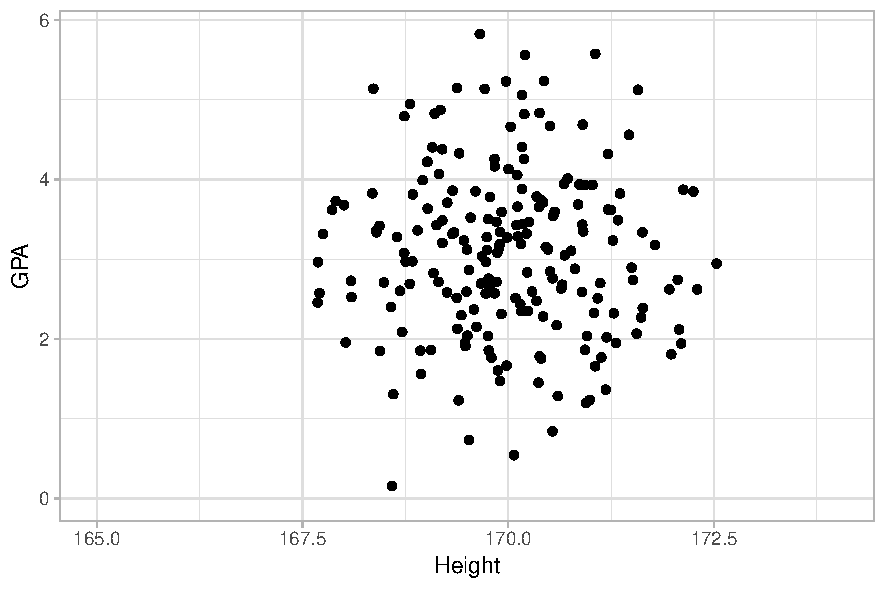
\includegraphics[width=0.8\linewidth]{../figs/class2/students_example0.pdf} \\[3mm]
    \visible<2>{Correlation: $0$}
\end{frame}

\begin{frame} \frametitle{Correlation Example}
    \centering
    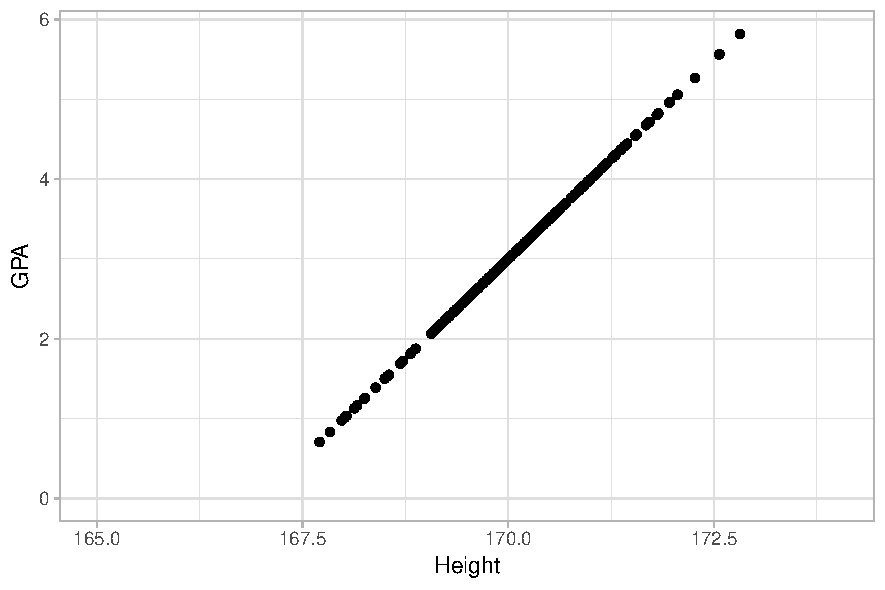
\includegraphics[width=0.8\linewidth]{../figs/class2/students_example1.pdf} \\[3mm]
    \visible<2>{Correlation: $1$}
\end{frame}

\begin{frame} \frametitle{Correlation Example}
    \centering
    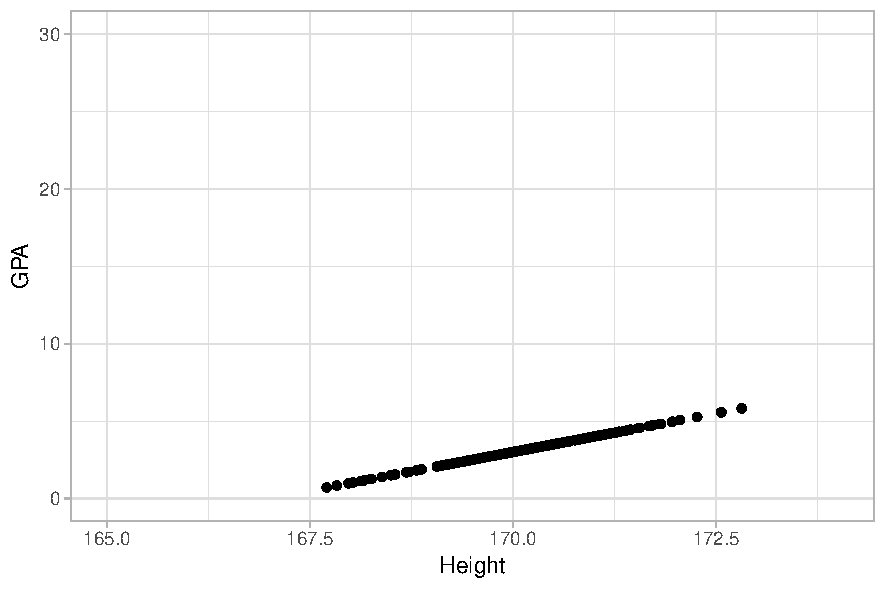
\includegraphics[width=0.8\linewidth]{../figs/class2/students_example1_stretched.pdf} \\[3mm]
    \visible<2>{Correlation: $1$}
\end{frame}

\begin{frame} \frametitle{Correlation Example}
    \centering
    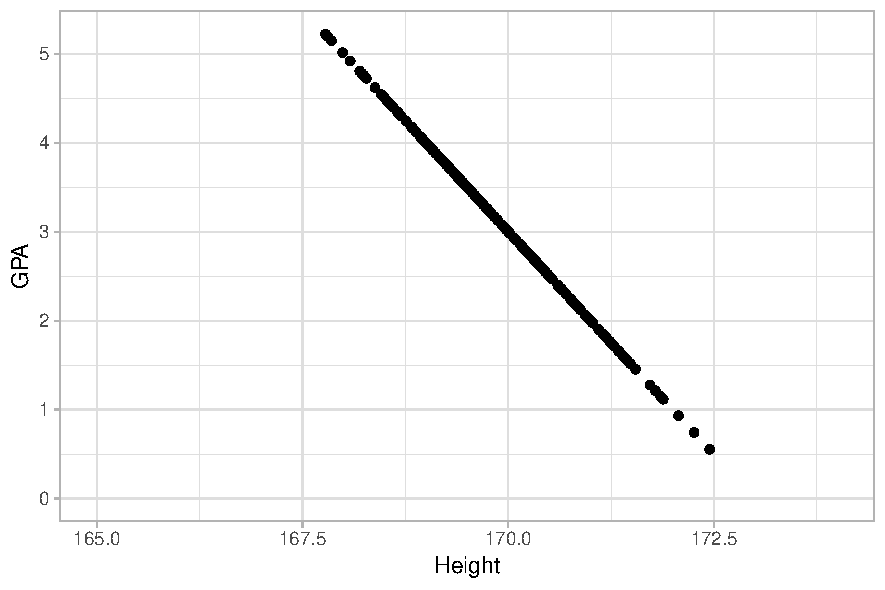
\includegraphics[width=0.8\linewidth]{../figs/class2/students_example2.pdf} \\[3mm]
    \visible<2>{Correlation: $-1$}
\end{frame}

\begin{frame} \frametitle{Correlation Example}
    \centering
    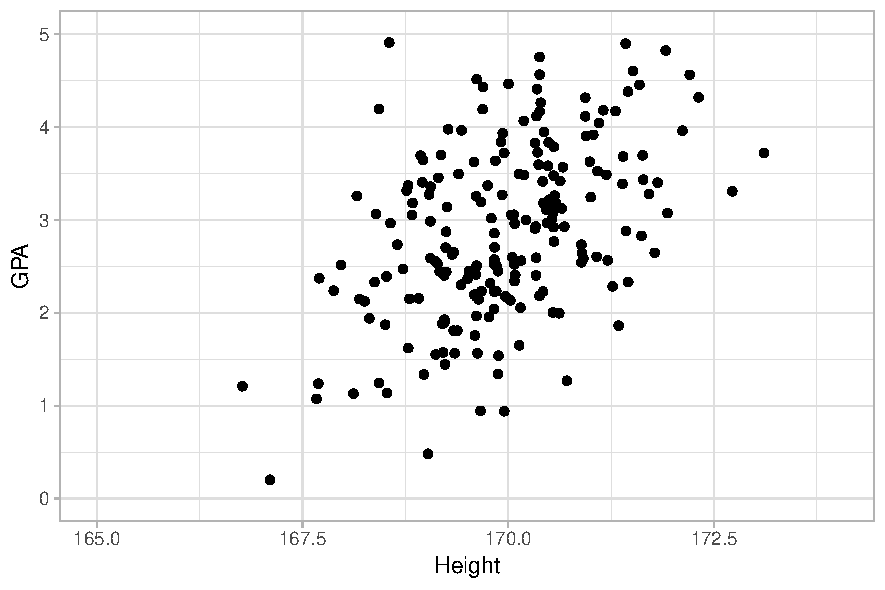
\includegraphics[width=0.8\linewidth]{../figs/class2/students_example3.pdf} \\[3mm]
    \visible<2>{Correlation: $0.5$}
\end{frame}

\begin{frame} \frametitle{Correlation Example}
    \centering
    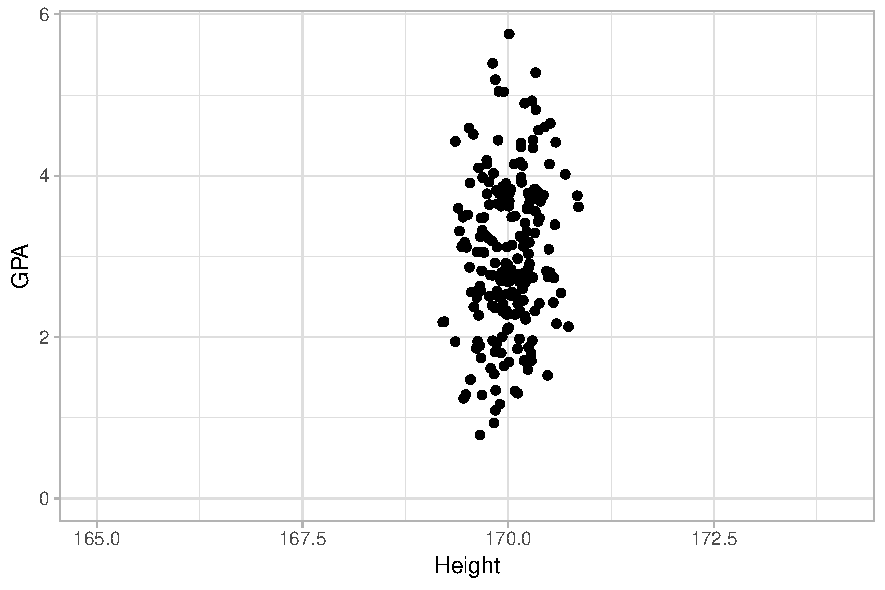
\includegraphics[width=0.8\linewidth]{../figs/class2/students_example4.pdf} \\[3mm]
    \visible<2>{Correlation: $0.0$}
\end{frame}


\begin{frame} \frametitle{Univariate Normal Distribution}
  Density for $X \sim \mathcal{N}(\mu , \sigma^2)$
  \[
   p(x \mid  \mu,\sigma^2) = \frac{1}{\sigma \sqrt{2\pi}} \exp \left( - \frac{(x-\mu)^2}{\sigma^2} \right)
 \]
 \begin{center}
   \includegraphics[width=0.7\linewidth]{../figs/prob/normal-univariate}
 \end{center}
\end{frame}

\begin{frame} \frametitle{Multivariate Normal Distribution}
  Joint probability density function
  \[
   p(x, y \mid  \bm{\mu}, \bm{\Sigma}) = \dots  
 \]
 \begin{center}
   \includegraphics[width=0.7\linewidth]{../figs/prob/normal-multivariate}
 \end{center}
\end{frame}

\begin{frame} \frametitle{Multivariate Normal Distribution}
  Joint probability density function
  \[
   p(x, y \mid  \bm{\mu}, \bm{\Sigma}) = \dots  
 \]
 \begin{center}
   \includegraphics[width=0.7\linewidth]{../figs/prob/normal-conditional}
 \end{center}
\end{frame}
\end{document}

%%% Local Variables:
%%% mode: latex
%%% TeX-master: t
%%% End: